%-----------------------------------------------------------------------------
% Example LaTeX template to be used for the Analytic Virtual Integration 
% of Cyber-Physical Systems Workshop (AVICPS).
%
% This template and related class-file (avicps.cls) is based on
% ACM SIGPLAN templates created by Paul C. Anagnostopoulos. The templates 
% are allowed to be used in the AVICPS workshop with permission from SIGPLAN 
% executive committee 2013. No other usage is permitted.
%
% The AVICPS version was created by David Broman
%-----------------------------------------------------------------------------

% Note: The output should be a PDF-file in A4 format. Recommended commands:
% > dvips -t a4 -o file.ps file.dvi
% > ps2pdf file.ps

\documentclass[10pt]{avicps} % Use file avicps.cls
                             % Use size 10pt for body text and A4 paper size.
                        
% Needed packages. Do not remove. The order of imported packages is important.
\usepackage{amsmath}
\usepackage{ae}                % Enables non-english letters, such as ���.
\usepackage{times}             % Using the times package, so that LaTeX and MS Word
                               %   look similar.
\usepackage{url}               % Handling of URL strings.
\usepackage[dvips]{graphicx}   % Include graphics.
                        
\begin{document}

\title{Paper Title}

% Use authorinfo, not normal \author
\authorinfo
{Author Name${}^1$ \quad Author Name${}^2$  \quad Author Name${}^1$}
{${}^1$Department, University, Country, $\texttt{\{name1,name3\}@university.org}$\\
 ${}^2$Company, Country, $\texttt{name2@company.com}$}
           
          
\maketitle
\begin{abstract}
This template gives the guidelines on how to prepare a paper for
submission to the Analytic Virtual Integration of Cyber-Physical
Systems Workshop (AVICPS).  Templates are available for both the LaTeX
and the Microsoft Word environment.  If there are any questions or
suggestions regarding this template, please send an email to
\verb|davbr@berkeley.edu|.
\end{abstract}

% Supply appropriate keywords for your article.
\keywords
keyword1, keyword2



%--------------------------------------------------------------------------------
\section{Introduction}

\subsection{Title and Authors}
The title should be centered using font \emph{Times New Roman} with
size 17pt. Words should be capitalized in the title, e.g., "This is an
Example of a Correct Title".

The author information should at least include name, affiliation
(department, university, country). Addresses and emails are optional
but strongly recommended.

\subsection{Abstract and Keywords}
The abstract should be written as one paragraph. It is not recommended
to exceed 150 words.
 
Appropriate keywords describing the content of the paper should be
supplied as a comma separated list.

\subsection{Fonts}
Use \emph{Times New Roman} with font size 10pt for the body text. To
emphasize a text or a word, use \emph{italic font
  style}. For~\verb|verbatim| text, including code examples, use the
\verb|\verb| command.


\subsection{Lists}


\begin{itemize}
\item The first text item.
\item The second text item.
\end{itemize}
    

\begin{enumerate}
\item The first text item.
\item The second text item.
\end{enumerate}

\subsection{Paragraphs}
The first paragraph after each subsection is not indented. When using
the \LaTeX~template, this is done automatically.

The second and following paragraphs within a section should be
indented.  In \LaTeX, this is done automatically.

\begin{figure}[b]
\centering
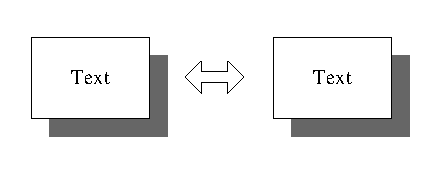
\includegraphics[width=0.4 \textwidth]{figure1}
\caption{An example of a figure that fits into one column.}
\label{fig:figure1}
\end{figure}

\begin{figure*}[t]
\centering
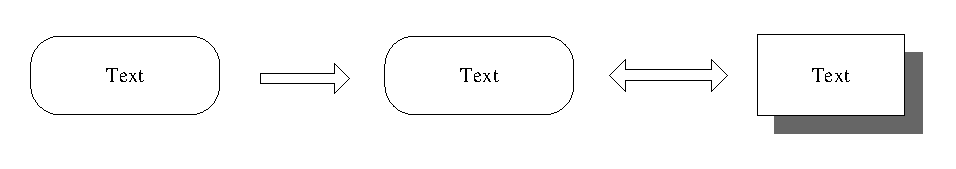
\includegraphics[width=0.9 \textwidth]{figure2}
\caption{Another example of a figure that spans over two columns.}
\label{fig:figure2}
\end{figure*}


%--------------------------------------------------------------------------------
\section{Section Headings}
Section headings should be numbered. Words in the headings should be
capatilized.

\subsection{Sub-Section} 
Subsections are numbered.

\subsubsection{Sub-Sub-Section}
It is possible to use sub-sub-sections. If possible, however, use only
sections and sub-sections.


%--------------------------------------------------------------------------------
\section{Figures}
Figures should be numbered and include a description text. All figures
should be referenced within the body text using the capitalized word
"Figure" followed by the figure number. For example,
Figure~\ref{fig:figure1} shows a figure located inside one column and
Figure~\ref{fig:figure2} illustrates how a figure can span over two
columns.

All figures should have a single line separating the figure and the
caption text\footnote{Footnotes should be numbered and located at the
  bottom of the column.}.


%--------------------------------------------------------------------------------
\section{Bibliographic References}
The bibliographic reference list should be shown at the end of the
paper, starting with an unnumbered heading \emph{"References"}. The
list of references should be sorted in alphabetic order according to
the first author's surname.

Citations are stated within the body text using the number of the
reference enclosed within brackets, e.g., \cite{Pantelides:1988}. If
more than one reference is cited at the same place, the list should be
sorted and within brackets, e.g.,
\cite{DuffReid:1978,Pierce:2002,Plotkin:1981}.


%--------------------------------------------------------------------------------
\section{Output Format}
The paper should be submitted as a PDF-file using page size A4 (not US
Letter!). All fonts should be included in the PDF-file.

Note: When using PDF-generators such as Adobe Acrobat PDF generator,
remember to enable high-quality output. If this option is not enabled,
figures and photos may be reduced in quality, resulting in poor
quality when printed.


%--------------------------------------------------------------------------------
% Acknowledgements
\acks The templates and instructions were created by David Broman.
The LaTeX template and related class file is based on ACM SIGPLAN
templates created by Paul C. Anagnostopoulos.  The LaTeX template is
allowed to be used in the AVICPS workshop with permission from SIGPLAN
executive committee 2013. No other usage is permitted.


%--------------------------------------------------------------------------------
% References using bibtex
\bibliographystyle{plain}
\bibliography{example}
\end{document}

